%!TEX root = farm.tex

\section{Platform Technology}\label{sec:tech}

First of all, we describe the platform technology underlying our
development.
We intensively focus on NVIDIA's GPU architectures, while the idea of
integrating GPU resource management into on-chip microcontrollers is not
limited to these specific architectures.
All pieces of technology presented herein are open-source, and may be
downloaded from the corresponding websites, respectively.

\subsection{Assembler for GPU microcontrollers}\label{sec:envy}

The assembler is comprised in package of the Envytools suite~\cite{envytools}.
The Envytools suite is a rich set of open-source tools to compile or
decompile GPU shader code, firmware code, macro code, and so on. 
It is also used to generate header files of GPU command definitions used
by the device driver and the runtime library.
There are many other useful tools and documentations for NVIDIA's GPU
architectures enclosed in the Envytools suite.

\subsection{GPU Device Driver}\label{sec:driver}

In general, the application programming interface (API) for the GPU is
provided by the runtime library.
GPU resource management, on the other hand, is often supported by the
device driver and the operating system (OS) module~\cite{Kato_ATC11,
Kato_ATC12, Bautin_MCNC08}.
As part of resource management, the device driver communicates with
microcontrollers integrated on the GPU.
The communication is typically managed by specific commands, which can
be handled by firmware running on each microcontroller.

\par
The firmware is built into the device driver by a shape of byte code,
and is uploaded on to the GPU at boot time.
To do so, we require open-source software, because we have to build the
firmware into the device driver.
In this paper, we use Gdev~\cite{Kato_ATC12}, an open-source module of
the GPGPU device driver and runtime library.

\subsection{LLVM Infrastructure}

The LLVM (Low Level Virtual Machine) project is a collection of
open-source modular and reusable compiler tool sets.
Since the microcontroller has its own instruction set architecture, we
develop an architecture-dependent backend of LLVM so that we can make
use of all the front-end modules of LLVM.

Figure \ref{fig:llvm} illustrates the structure of LLVM.
It first generates the LLVM IR (Intermediate Representation) from the
source code. 
This IR code is assembled by the LLVM backend.
The assembly code is finally translated to the object code for the
target machine.

\begin{figure}
\begin{center}
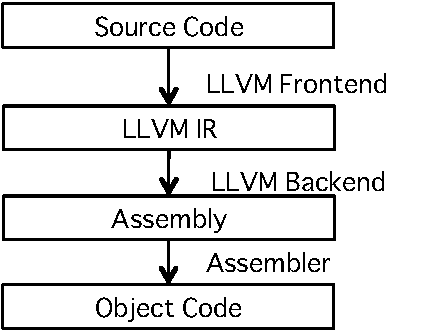
\includegraphics[scale = 0.5]{./img/llvmflow.pdf}
\end{center}
\caption{Compilation stages of LLVM.}
\label{fig:llvm}
\end{figure}

\subsubsection{LLVM IR}

The LLVM IR is an intermediate language used in LLVM, also called bitcode or
LLVM assembly languages.
This intermediate language is very powerful, scalable, light-weight, and
low-level enough to underlie many languages on top of many
architectures.
LLVM uses an expression of SSA (Static Single Assignment), which is
suitable for a lot of compiler optimization algorithms.

\subsubsection{LLVM frontend}\label{set:clang}

The LLVM frontend generates an intermediate language from a high-level
language in LLVM.
It is mainly used for code generation and its optimization.
In particular, we use Clang for our development, which is an open-source
compiler for the C family of programming languages provided by LLVM.

\subsubsection{LLVM backend}\label{set:backend}

The LLVM backend generates target code from an intermediate language in
LLVM.
The backend of LLVM features a target-independent code generator that
may create output for several types of target processors including X86,
PowerPC, ARM, and SPARC. 
This backend framework may also be used to generate code targeted at
accelerators such as Cell B/E and GPUs.
In fact, NVIDIA has announced recently that they use LLVM for the basis
of their CUDA compiler.
The backend of LLVM is composed of the LLC (LLVM static Compiler) and
the LLI (LLVM Interpreter).
LLI is an interpreter of the LLVM IR, also available as a JIT compiler,
while LLC is a static compiler to generate code.
We use this backend part of LLVM to generate code targeted at NVIDIA's
GPU microcontrollers.

